\documentclass[1p]{elsarticle_modified}
%\bibliographystyle{elsarticle-num}

%\usepackage[colorlinks]{hyperref}
%\usepackage{abbrmath_seonhwa} %\Abb, \Ascr, \Acal ,\Abf, \Afrak
\usepackage{amsfonts}
\usepackage{amssymb}
\usepackage{amsmath}
\usepackage{amsthm}
\usepackage{scalefnt}
\usepackage{amsbsy}
\usepackage{kotex}
\usepackage{caption}
\usepackage{subfig}
\usepackage{color}
\usepackage{graphicx}
\usepackage{xcolor} %% white, black, red, green, blue, cyan, magenta, yellow
\usepackage{float}
\usepackage{setspace}
\usepackage{hyperref}

\usepackage{tikz}
\usetikzlibrary{arrows}

\usepackage{multirow}
\usepackage{array} % fixed length table
\usepackage{hhline}

%%%%%%%%%%%%%%%%%%%%%
\makeatletter
\renewcommand*\env@matrix[1][\arraystretch]{%
	\edef\arraystretch{#1}%
	\hskip -\arraycolsep
	\let\@ifnextchar\new@ifnextchar
	\array{*\c@MaxMatrixCols c}}
\makeatother %https://tex.stackexchange.com/questions/14071/how-can-i-increase-the-line-spacing-in-a-matrix
%%%%%%%%%%%%%%%

\usepackage[normalem]{ulem}

\newcommand{\msout}[1]{\ifmmode\text{\sout{\ensuremath{#1}}}\else\sout{#1}\fi}
%SOURCE: \msout is \stkout macro in https://tex.stackexchange.com/questions/20609/strikeout-in-math-mode

\newcommand{\cancel}[1]{
	\ifmmode
	{\color{red}\msout{#1}}
	\else
	{\color{red}\sout{#1}}
	\fi
}

\newcommand{\add}[1]{
	{\color{blue}\uwave{#1}}
}

\newcommand{\replace}[2]{
	\ifmmode
	{\color{red}\msout{#1}}{\color{blue}\uwave{#2}}
	\else
	{\color{red}\sout{#1}}{\color{blue}\uwave{#2}}
	\fi
}

\newcommand{\Sol}{\mathcal{S}} %segment
\newcommand{\D}{D} %diagram
\newcommand{\A}{\mathcal{A}} %arc


%%%%%%%%%%%%%%%%%%%%%%%%%%%%%5 test

\def\sl{\operatorname{\textup{SL}}(2,\Cbb)}
\def\psl{\operatorname{\textup{PSL}}(2,\Cbb)}
\def\quan{\mkern 1mu \triangleright \mkern 1mu}

\theoremstyle{definition}
\newtheorem{thm}{Theorem}[section]
\newtheorem{prop}[thm]{Proposition}
\newtheorem{lem}[thm]{Lemma}
\newtheorem{ques}[thm]{Question}
\newtheorem{cor}[thm]{Corollary}
\newtheorem{defn}[thm]{Definition}
\newtheorem{exam}[thm]{Example}
\newtheorem{rmk}[thm]{Remark}
\newtheorem{alg}[thm]{Algorithm}

\newcommand{\I}{\sqrt{-1}}
\begin{document}

%\begin{frontmatter}
%
%\title{Boundary parabolic representations of knots up to 8 crossings}
%
%%% Group authors per affiliation:
%\author{Yunhi Cho} 
%\address{Department of Mathematics, University of Seoul, Seoul, Korea}
%\ead{yhcho@uos.ac.kr}
%
%
%\author{Seonhwa Kim} %\fnref{s_kim}}
%\address{Center for Geometry and Physics, Institute for Basic Science, Pohang, 37673, Korea}
%\ead{ryeona17@ibs.re.kr}
%
%\author{Hyuk Kim}
%\address{Department of Mathematical Sciences, Seoul National University, Seoul 08826, Korea}
%\ead{hyukkim@snu.ac.kr}
%
%\author{Seokbeom Yoon}
%\address{Department of Mathematical Sciences, Seoul National University, Seoul, 08826,  Korea}
%\ead{sbyoon15@snu.ac.kr}
%
%\begin{abstract}
%We find all boundary parabolic representation of knots up to 8 crossings.
%
%\end{abstract}
%\begin{keyword}
%    \MSC[2010] 57M25 
%\end{keyword}
%
%\end{frontmatter}

%\linenumbers
%\tableofcontents
%
\newcommand\colored[1]{\textcolor{white}{\rule[-0.35ex]{0.8em}{1.4ex}}\kern-0.8em\color{red} #1}%
%\newcommand\colored[1]{\textcolor{white}{ #1}\kern-2.17ex	\textcolor{white}{ #1}\kern-1.81ex	\textcolor{white}{ #1}\kern-2.15ex\color{red}#1	}

{\Large $\underline{12n_{0097}~(K12n_{0097})}$}

\setlength{\tabcolsep}{10pt}
\renewcommand{\arraystretch}{1.6}
\vspace{1cm}\begin{tabular}{m{100pt}>{\centering\arraybackslash}m{274pt}}
\multirow{5}{120pt}{
	\centering
	\includegraphics[width=112pt]{../../../GIT/diagram.site/Diagrams/png/2186_12n_0097.png}\\
\ \ \ A knot diagram\footnotemark}&
\allowdisplaybreaks
\textbf{Linearized knot diagam} \\
\cline{2-2}
 &
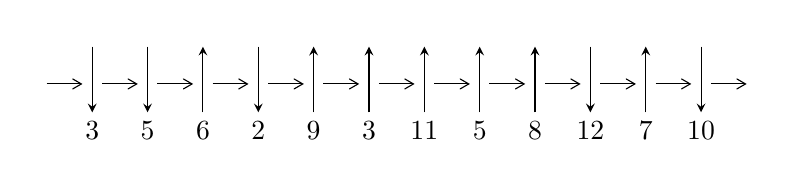
\begin{tikzpicture}[x=20pt, y=17pt]
	% nodes
	\node (C0) at (0, 0) {};
	\node (C1) at (1, 0) {};
	\node (C1U) at (1, +1) {};
	\node (C1D) at (1, -1) {3};

	\node (C2) at (2, 0) {};
	\node (C2U) at (2, +1) {};
	\node (C2D) at (2, -1) {5};

	\node (C3) at (3, 0) {};
	\node (C3U) at (3, +1) {};
	\node (C3D) at (3, -1) {6};

	\node (C4) at (4, 0) {};
	\node (C4U) at (4, +1) {};
	\node (C4D) at (4, -1) {2};

	\node (C5) at (5, 0) {};
	\node (C5U) at (5, +1) {};
	\node (C5D) at (5, -1) {9};

	\node (C6) at (6, 0) {};
	\node (C6U) at (6, +1) {};
	\node (C6D) at (6, -1) {3};

	\node (C7) at (7, 0) {};
	\node (C7U) at (7, +1) {};
	\node (C7D) at (7, -1) {11};

	\node (C8) at (8, 0) {};
	\node (C8U) at (8, +1) {};
	\node (C8D) at (8, -1) {5};

	\node (C9) at (9, 0) {};
	\node (C9U) at (9, +1) {};
	\node (C9D) at (9, -1) {8};

	\node (C10) at (10, 0) {};
	\node (C10U) at (10, +1) {};
	\node (C10D) at (10, -1) {12};

	\node (C11) at (11, 0) {};
	\node (C11U) at (11, +1) {};
	\node (C11D) at (11, -1) {7};

	\node (C12) at (12, 0) {};
	\node (C12U) at (12, +1) {};
	\node (C12D) at (12, -1) {10};
	\node (C13) at (13, 0) {};

	% arrows
	\draw[->,>={angle 60}]
	(C0) edge (C1) (C1) edge (C2) (C2) edge (C3) (C3) edge (C4) (C4) edge (C5) (C5) edge (C6) (C6) edge (C7) (C7) edge (C8) (C8) edge (C9) (C9) edge (C10) (C10) edge (C11) (C11) edge (C12) (C12) edge (C13) ;	\draw[->,>=stealth]
	(C1U) edge (C1D) (C2U) edge (C2D) (C3D) edge (C3U) (C4U) edge (C4D) (C5D) edge (C5U) (C6D) edge (C6U) (C7D) edge (C7U) (C8D) edge (C8U) (C9D) edge (C9U) (C10U) edge (C10D) (C11D) edge (C11U) (C12U) edge (C12D) ;
	\end{tikzpicture} \\
\hhline{~~} \\& 
\textbf{Solving Sequence} \\ \cline{2-2} 
 &
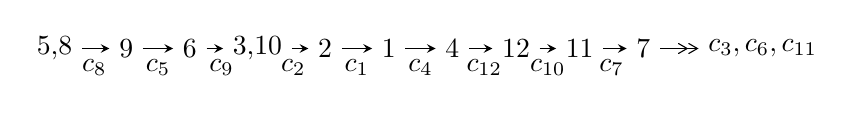
\begin{tikzpicture}[x=23pt, y=7pt]
	% node
	\node (A0) at (-1/8, 0) {5,8};
	\node (A1) at (1, 0) {9};
	\node (A2) at (2, 0) {6};
	\node (A3) at (49/16, 0) {3,10};
	\node (A4) at (33/8, 0) {2};
	\node (A5) at (41/8, 0) {1};
	\node (A6) at (49/8, 0) {4};
	\node (A7) at (57/8, 0) {12};
	\node (A8) at (65/8, 0) {11};
	\node (A9) at (73/8, 0) {7};
	\node (C1) at (1/2, -1) {$c_{8}$};
	\node (C2) at (3/2, -1) {$c_{5}$};
	\node (C3) at (5/2, -1) {$c_{9}$};
	\node (C4) at (29/8, -1) {$c_{2}$};
	\node (C5) at (37/8, -1) {$c_{1}$};
	\node (C6) at (45/8, -1) {$c_{4}$};
	\node (C7) at (53/8, -1) {$c_{12}$};
	\node (C8) at (61/8, -1) {$c_{10}$};
	\node (C9) at (69/8, -1) {$c_{7}$};
	\node (A10) at (11, 0) {$c_{3},c_{6},c_{11}$};

	% edge
	\draw[->,>=stealth]	
	(A0) edge (A1) (A1) edge (A2) (A2) edge (A3) (A3) edge (A4) (A4) edge (A5) (A5) edge (A6) (A6) edge (A7) (A7) edge (A8) (A8) edge (A9) ;
	\draw[->>,>={angle 60}]	
	(A9) edge (A10);
\end{tikzpicture} \\ 

\end{tabular} \\

\footnotetext{
The image of knot diagram is generated by the software ``\textbf{Draw programme}" developed by Andrew Bartholomew(\url{http://www.layer8.co.uk/maths/draw/index.htm\#Running-draw}), where we modified some parts for our purpose(\url{https://github.com/CATsTAILs/LinksPainter}).
}\phantom \\ \newline 
\centering \textbf{Ideals for irreducible components\footnotemark of $X_{\text{par}}$} 
 
\begin{align*}
I^u_{1}&=\langle 
-1.08330\times10^{15} u^{28}+2.63231\times10^{15} u^{27}+\cdots+2.88806\times10^{15} b-3.18100\times10^{15},\\
\phantom{I^u_{1}}&\phantom{= \langle  }-1.08330\times10^{15} u^{28}+2.63231\times10^{15} u^{27}+\cdots+2.88806\times10^{15} a-3.18100\times10^{15},\;u^{29}-2 u^{28}+\cdots+u-1\rangle \\
I^u_{2}&=\langle 
- u^8- u^7+2 u^6+3 u^5- u^4-3 u^3-2 u^2+b+u+1,\;- u^8- u^7+2 u^6+3 u^5- u^4-3 u^3-2 u^2+a+1,\\
\phantom{I^u_{2}}&\phantom{= \langle  }u^9+u^8-2 u^7-3 u^6+u^5+3 u^4+2 u^3- u-1\rangle \\
\\
\end{align*}
\raggedright * 2 irreducible components of $\dim_{\mathbb{C}}=0$, with total 38 representations.\\
\footnotetext{All coefficients of polynomials are rational numbers. But the coefficients are sometimes approximated in decimal forms when there is not enough margin.}
\newpage
\renewcommand{\arraystretch}{1}
\centering \section*{I. $I^u_{1}= \langle -1.08\times10^{15} u^{28}+2.63\times10^{15} u^{27}+\cdots+2.89\times10^{15} b-3.18\times10^{15},\;-1.08\times10^{15} u^{28}+2.63\times10^{15} u^{27}+\cdots+2.89\times10^{15} a-3.18\times10^{15},\;u^{29}-2 u^{28}+\cdots+u-1 \rangle$}
\flushleft \textbf{(i) Arc colorings}\\
\begin{tabular}{m{7pt} m{180pt} m{7pt} m{180pt} }
\flushright $a_{5}=$&$\begin{pmatrix}0\\u\end{pmatrix}$ \\
\flushright $a_{8}=$&$\begin{pmatrix}1\\0\end{pmatrix}$ \\
\flushright $a_{9}=$&$\begin{pmatrix}1\\- u^2\end{pmatrix}$ \\
\flushright $a_{6}=$&$\begin{pmatrix}u\\- u^3+u\end{pmatrix}$ \\
\flushright $a_{3}=$&$\begin{pmatrix}0.375096 u^{28}-0.911447 u^{27}+\cdots-0.238354 u+1.10143\\0.375096 u^{28}-0.911447 u^{27}+\cdots+0.761646 u+1.10143\end{pmatrix}$ \\
\flushright $a_{10}=$&$\begin{pmatrix}- u^2+1\\- u^2\end{pmatrix}$ \\
\flushright $a_{2}=$&$\begin{pmatrix}0.375096 u^{28}-0.911447 u^{27}+\cdots-0.238354 u+1.10143\\0.240332 u^{28}-0.538132 u^{27}+\cdots+0.225295 u+1.26269\end{pmatrix}$ \\
\flushright $a_{1}=$&$\begin{pmatrix}0.360721 u^{28}-0.778371 u^{27}+\cdots-0.736984 u+0.338038\\0.0965394 u^{28}-0.0157569 u^{27}+\cdots-0.674515 u+0.641092\end{pmatrix}$ \\
\flushright $a_{4}=$&$\begin{pmatrix}0.259382 u^{28}-0.660563 u^{27}+\cdots+0.000197369 u+0.997644\\0.264728 u^{28}-0.644578 u^{27}+\cdots+1.13537 u+0.978187\end{pmatrix}$ \\
\flushright $a_{12}=$&$\begin{pmatrix}-0.0381007 u^{28}+0.244861 u^{27}+\cdots-0.549804 u+0.530085\\-0.153814 u^{28}+0.495745 u^{27}+\cdots-0.311253 u+0.426298\end{pmatrix}$ \\
\flushright $a_{11}=$&$\begin{pmatrix}0.00860430 u^{28}-0.157377 u^{27}+\cdots+0.318117 u-0.890976\\-0.00366395 u^{28}-0.0860215 u^{27}+\cdots+0.240983 u-1.25230\end{pmatrix}$ \\
\flushright $a_{7}=$&$\begin{pmatrix}-0.264182 u^{28}+0.762614 u^{27}+\cdots+0.0624682 u+0.303054\\-0.148468 u^{28}+0.511730 u^{27}+\cdots-0.176083 u+0.406841\end{pmatrix}$\\&\end{tabular}
\flushleft \textbf{(ii) Obstruction class $= -1$}\\~\\
\flushleft \textbf{(iii) Cusp Shapes $= \frac{16119990594582668}{2888060083449331} u^{28}-\frac{28126461598340071}{2888060083449331} u^{27}+\cdots+\frac{17982394285452960}{2888060083449331} u+\frac{11832001216098990}{2888060083449331}$}\\~\\
\newpage\renewcommand{\arraystretch}{1}
\flushleft \textbf{(iv) u-Polynomials at the component}\newline \\
\begin{tabular}{m{50pt}|m{274pt}}
Crossings & \hspace{64pt}u-Polynomials at each crossing \\
\hline $$\begin{aligned}c_{1}\end{aligned}$$&$\begin{aligned}
&u^{29}+48 u^{28}+\cdots+79 u+1
\end{aligned}$\\
\hline $$\begin{aligned}c_{2},c_{4}\end{aligned}$$&$\begin{aligned}
&u^{29}-10 u^{28}+\cdots+19 u-1
\end{aligned}$\\
\hline $$\begin{aligned}c_{3},c_{6}\end{aligned}$$&$\begin{aligned}
&u^{29}+5 u^{28}+\cdots+1536 u-512
\end{aligned}$\\
\hline $$\begin{aligned}c_{5},c_{8}\end{aligned}$$&$\begin{aligned}
&u^{29}-2 u^{28}+\cdots+u-1
\end{aligned}$\\
\hline $$\begin{aligned}c_{7},c_{11}\end{aligned}$$&$\begin{aligned}
&u^{29}+2 u^{28}+\cdots- u-1
\end{aligned}$\\
\hline $$\begin{aligned}c_{9}\end{aligned}$$&$\begin{aligned}
&u^{29}+30 u^{27}+\cdots- u-1
\end{aligned}$\\
\hline $$\begin{aligned}c_{10},c_{12}\end{aligned}$$&$\begin{aligned}
&u^{29}+12 u^{28}+\cdots- u-1
\end{aligned}$\\
\hline
\end{tabular}\\~\\
\newpage\renewcommand{\arraystretch}{1}
\flushleft \textbf{(v) Riley Polynomials at the component}\newline \\
\begin{tabular}{m{50pt}|m{274pt}}
Crossings & \hspace{64pt}Riley Polynomials at each crossing \\
\hline $$\begin{aligned}c_{1}\end{aligned}$$&$\begin{aligned}
&y^{29}-124 y^{28}+\cdots-7313 y-1
\end{aligned}$\\
\hline $$\begin{aligned}c_{2},c_{4}\end{aligned}$$&$\begin{aligned}
&y^{29}-48 y^{28}+\cdots+79 y-1
\end{aligned}$\\
\hline $$\begin{aligned}c_{3},c_{6}\end{aligned}$$&$\begin{aligned}
&y^{29}+57 y^{28}+\cdots+3932160 y-262144
\end{aligned}$\\
\hline $$\begin{aligned}c_{5},c_{8}\end{aligned}$$&$\begin{aligned}
&y^{29}+30 y^{27}+\cdots- y-1
\end{aligned}$\\
\hline $$\begin{aligned}c_{7},c_{11}\end{aligned}$$&$\begin{aligned}
&y^{29}+12 y^{28}+\cdots- y-1
\end{aligned}$\\
\hline $$\begin{aligned}c_{9}\end{aligned}$$&$\begin{aligned}
&y^{29}+60 y^{28}+\cdots-5 y-1
\end{aligned}$\\
\hline $$\begin{aligned}c_{10},c_{12}\end{aligned}$$&$\begin{aligned}
&y^{29}+12 y^{28}+\cdots+19 y-1
\end{aligned}$\\
\hline
\end{tabular}\\~\\
\newpage\flushleft \textbf{(vi) Complex Volumes and Cusp Shapes}
$$\begin{array}{c|c|c}  
\text{Solutions to }I^u_{1}& \I (\text{vol} + \sqrt{-1}CS) & \text{Cusp shape}\\
 \hline 
\begin{aligned}
u &= \phantom{-}0.365827 + 0.867755 I \\
a &= -0.58586 - 1.71900 I \\
b &= -0.220028 - 0.851246 I\end{aligned}
 & -3.76536 + 5.51790 I & -3.77377 - 7.24287 I \\ \hline\begin{aligned}
u &= \phantom{-}0.365827 - 0.867755 I \\
a &= -0.58586 + 1.71900 I \\
b &= -0.220028 + 0.851246 I\end{aligned}
 & -3.76536 - 5.51790 I & -3.77377 + 7.24287 I \\ \hline\begin{aligned}
u &= \phantom{-}1.038780 + 0.399171 I \\
a &= -0.532542 - 0.137121 I \\
b &= \phantom{-}0.506240 + 0.262051 I\end{aligned}
 & \phantom{-}3.61222 + 0.74335 I & \phantom{-}9.35759 + 0.47912 I \\ \hline\begin{aligned}
u &= \phantom{-}1.038780 - 0.399171 I \\
a &= -0.532542 + 0.137121 I \\
b &= \phantom{-}0.506240 - 0.262051 I\end{aligned}
 & \phantom{-}3.61222 - 0.74335 I & \phantom{-}9.35759 - 0.47912 I \\ \hline\begin{aligned}
u &= \phantom{-}0.149316 + 0.856366 I \\
a &= -0.21482 - 2.05855 I \\
b &= -0.065503 - 1.202180 I\end{aligned}
 & -4.88663 - 0.95031 I & -6.59475 + 1.19001 I \\ \hline\begin{aligned}
u &= \phantom{-}0.149316 - 0.856366 I \\
a &= -0.21482 + 2.05855 I \\
b &= -0.065503 + 1.202180 I\end{aligned}
 & -4.88663 + 0.95031 I & -6.59475 - 1.19001 I \\ \hline\begin{aligned}
u &= -1.024520 + 0.534163 I \\
a &= \phantom{-}0.624645 - 0.175606 I \\
b &= -0.399874 + 0.358557 I\end{aligned}
 & \phantom{-}2.77162 - 6.24281 I & \phantom{-}6.28797 + 4.80418 I \\ \hline\begin{aligned}
u &= -1.024520 - 0.534163 I \\
a &= \phantom{-}0.624645 + 0.175606 I \\
b &= -0.399874 - 0.358557 I\end{aligned}
 & \phantom{-}2.77162 + 6.24281 I & \phantom{-}6.28797 - 4.80418 I \\ \hline\begin{aligned}
u &= -0.350587 + 0.709669 I \\
a &= \phantom{-}0.21366 - 1.51930 I \\
b &= -0.136928 - 0.809633 I\end{aligned}
 & -1.85641 - 1.40408 I & -0.21276 + 2.68754 I \\ \hline\begin{aligned}
u &= -0.350587 - 0.709669 I \\
a &= \phantom{-}0.21366 + 1.51930 I \\
b &= -0.136928 + 0.809633 I\end{aligned}
 & -1.85641 + 1.40408 I & -0.21276 - 2.68754 I\\
 \hline 
 \end{array}$$\newpage$$\begin{array}{c|c|c}  
\text{Solutions to }I^u_{1}& \I (\text{vol} + \sqrt{-1}CS) & \text{Cusp shape}\\
 \hline 
\begin{aligned}
u &= -0.563294 + 0.524681 I \\
a &= \phantom{-}0.170413 - 0.678152 I \\
b &= -0.392881 - 0.153472 I\end{aligned}
 & -1.43698 - 1.52178 I & -1.26786 + 4.70761 I \\ \hline\begin{aligned}
u &= -0.563294 - 0.524681 I \\
a &= \phantom{-}0.170413 + 0.678152 I \\
b &= -0.392881 + 0.153472 I\end{aligned}
 & -1.43698 + 1.52178 I & -1.26786 - 4.70761 I \\ \hline\begin{aligned}
u &= \phantom{-}0.702050\phantom{ +0.000000I} \\
a &= -0.244600\phantom{ +0.000000I} \\
b &= \phantom{-}0.457450\phantom{ +0.000000I}\end{aligned}
 & \phantom{-}0.941539\phantom{ +0.000000I} & \phantom{-}11.3890\phantom{ +0.000000I} \\ \hline\begin{aligned}
u &= -0.121762 + 0.604163 I \\
a &= -0.084430 + 0.174292 I \\
b &= -0.206192 + 0.778455 I\end{aligned}
 & \phantom{-}0.47173 + 2.34023 I & \phantom{-}2.64159 - 2.77169 I \\ \hline\begin{aligned}
u &= -0.121762 - 0.604163 I \\
a &= -0.084430 - 0.174292 I \\
b &= -0.206192 - 0.778455 I\end{aligned}
 & \phantom{-}0.47173 - 2.34023 I & \phantom{-}2.64159 + 2.77169 I \\ \hline\begin{aligned}
u &= -0.444471 + 0.402241 I \\
a &= -0.957420 - 0.680211 I \\
b &= -1.40189 - 0.27797 I\end{aligned}
 & -1.17268 - 1.39986 I & -2.59264 + 6.14012 I \\ \hline\begin{aligned}
u &= -0.444471 - 0.402241 I \\
a &= -0.957420 + 0.680211 I \\
b &= -1.40189 + 0.27797 I\end{aligned}
 & -1.17268 + 1.39986 I & -2.59264 - 6.14012 I \\ \hline\begin{aligned}
u &= \phantom{-}0.508912 + 0.193701 I \\
a &= \phantom{-}1.88309 - 0.38641 I \\
b &= \phantom{-}2.39201 - 0.19271 I\end{aligned}
 & -1.87493 - 2.49067 I & \phantom{-}4.89703 - 8.29090 I \\ \hline\begin{aligned}
u &= \phantom{-}0.508912 - 0.193701 I \\
a &= \phantom{-}1.88309 + 0.38641 I \\
b &= \phantom{-}2.39201 + 0.19271 I\end{aligned}
 & -1.87493 + 2.49067 I & \phantom{-}4.89703 + 8.29090 I \\ \hline\begin{aligned}
u &= \phantom{-}1.07631 + 1.11196 I \\
a &= -0.679049 + 1.085630 I \\
b &= \phantom{-}0.39726 + 2.19758 I\end{aligned}
 & -14.1601 + 12.3738 I & -0.83426 - 6.38685 I\\
 \hline 
 \end{array}$$\newpage$$\begin{array}{c|c|c}  
\text{Solutions to }I^u_{1}& \I (\text{vol} + \sqrt{-1}CS) & \text{Cusp shape}\\
 \hline 
\begin{aligned}
u &= \phantom{-}1.07631 - 1.11196 I \\
a &= -0.679049 - 1.085630 I \\
b &= \phantom{-}0.39726 - 2.19758 I\end{aligned}
 & -14.1601 - 12.3738 I & -0.83426 + 6.38685 I \\ \hline\begin{aligned}
u &= -1.08388 + 1.11855 I \\
a &= \phantom{-}0.705879 + 1.020200 I \\
b &= -0.37800 + 2.13875 I\end{aligned}
 & -12.19450 - 6.48359 I & \phantom{-}1.17949 + 2.27770 I \\ \hline\begin{aligned}
u &= -1.08388 - 1.11855 I \\
a &= \phantom{-}0.705879 - 1.020200 I \\
b &= -0.37800 - 2.13875 I\end{aligned}
 & -12.19450 + 6.48359 I & \phantom{-}1.17949 - 2.27770 I \\ \hline\begin{aligned}
u &= \phantom{-}1.09561 + 1.10785 I \\
a &= -0.847927 + 1.022520 I \\
b &= \phantom{-}0.24768 + 2.13037 I\end{aligned}
 & -18.7416 + 4.0694 I & -3.78877 - 1.98533 I \\ \hline\begin{aligned}
u &= \phantom{-}1.09561 - 1.10785 I \\
a &= -0.847927 - 1.022520 I \\
b &= \phantom{-}0.24768 - 2.13037 I\end{aligned}
 & -18.7416 - 4.0694 I & -3.78877 + 1.98533 I \\ \hline\begin{aligned}
u &= \phantom{-}1.11251 + 1.10380 I \\
a &= -0.923170 + 0.842832 I \\
b &= \phantom{-}0.18934 + 1.94663 I\end{aligned}
 & -14.0670 - 4.2413 I & -1.00950 + 2.34740 I \\ \hline\begin{aligned}
u &= \phantom{-}1.11251 - 1.10380 I \\
a &= -0.923170 - 0.842832 I \\
b &= \phantom{-}0.18934 - 1.94663 I\end{aligned}
 & -14.0670 + 4.2413 I & -1.00950 - 2.34740 I \\ \hline\begin{aligned}
u &= -1.10978 + 1.11274 I \\
a &= \phantom{-}0.849824 + 0.873104 I \\
b &= -0.25996 + 1.98584 I\end{aligned}
 & -12.12700 - 1.69249 I & \phantom{-}1.01629 + 1.84111 I \\ \hline\begin{aligned}
u &= -1.10978 - 1.11274 I \\
a &= \phantom{-}0.849824 - 0.873104 I \\
b &= -0.25996 - 1.98584 I\end{aligned}
 & -12.12700 + 1.69249 I & \phantom{-}1.01629 - 1.84111 I\\
 \hline 
 \end{array}$$\newpage\newpage\renewcommand{\arraystretch}{1}
\centering \section*{II. $I^u_{2}= \langle - u^8- u^7+\cdots+b+1,\;- u^8- u^7+\cdots+a+1,\;u^9+u^8-2 u^7-3 u^6+u^5+3 u^4+2 u^3- u-1 \rangle$}
\flushleft \textbf{(i) Arc colorings}\\
\begin{tabular}{m{7pt} m{180pt} m{7pt} m{180pt} }
\flushright $a_{5}=$&$\begin{pmatrix}0\\u\end{pmatrix}$ \\
\flushright $a_{8}=$&$\begin{pmatrix}1\\0\end{pmatrix}$ \\
\flushright $a_{9}=$&$\begin{pmatrix}1\\- u^2\end{pmatrix}$ \\
\flushright $a_{6}=$&$\begin{pmatrix}u\\- u^3+u\end{pmatrix}$ \\
\flushright $a_{3}=$&$\begin{pmatrix}u^8+u^7-2 u^6-3 u^5+u^4+3 u^3+2 u^2-1\\u^8+u^7-2 u^6-3 u^5+u^4+3 u^3+2 u^2- u-1\end{pmatrix}$ \\
\flushright $a_{10}=$&$\begin{pmatrix}- u^2+1\\- u^2\end{pmatrix}$ \\
\flushright $a_{2}=$&$\begin{pmatrix}u^8+u^7-2 u^6-3 u^5+u^4+3 u^3+2 u^2-1\\u^8+u^7-2 u^6-3 u^5+u^4+3 u^3+2 u^2-2 u-1\end{pmatrix}$ \\
\flushright $a_{1}=$&$\begin{pmatrix}0\\- u\end{pmatrix}$ \\
\flushright $a_{4}=$&$\begin{pmatrix}u^8+u^7-2 u^6-3 u^5+u^4+3 u^3+2 u^2-1\\u^8+u^7-2 u^6-3 u^5+u^4+3 u^3+2 u^2- u-1\end{pmatrix}$ \\
\flushright $a_{12}=$&$\begin{pmatrix}- u^5+2 u^3- u\\- u^5+u^3- u\end{pmatrix}$ \\
\flushright $a_{11}=$&$\begin{pmatrix}- u^8+3 u^6-3 u^4+1\\- u^8+2 u^6-2 u^4\end{pmatrix}$ \\
\flushright $a_{7}=$&$\begin{pmatrix}u\\- u^3+u\end{pmatrix}$\\&\end{tabular}
\flushleft \textbf{(ii) Obstruction class $= 1$}\\~\\
\flushleft \textbf{(iii) Cusp Shapes $= - u^8+2 u^7+2 u^6-3 u^5-6 u^4+3 u^3+3 u^2+4 u-2$}\\~\\
\newpage\renewcommand{\arraystretch}{1}
\flushleft \textbf{(iv) u-Polynomials at the component}\newline \\
\begin{tabular}{m{50pt}|m{274pt}}
Crossings & \hspace{64pt}u-Polynomials at each crossing \\
\hline $$\begin{aligned}c_{1},c_{2}\end{aligned}$$&$\begin{aligned}
&(u-1)^9
\end{aligned}$\\
\hline $$\begin{aligned}c_{3},c_{6}\end{aligned}$$&$\begin{aligned}
&u^9
\end{aligned}$\\
\hline $$\begin{aligned}c_{4}\end{aligned}$$&$\begin{aligned}
&(u+1)^9
\end{aligned}$\\
\hline $$\begin{aligned}c_{5}\end{aligned}$$&$\begin{aligned}
&u^9- u^8-2 u^7+3 u^6+u^5-3 u^4+2 u^3- u+1
\end{aligned}$\\
\hline $$\begin{aligned}c_{7}\end{aligned}$$&$\begin{aligned}
&u^9- u^8+2 u^7- u^6+3 u^5- u^4+2 u^3+u+1
\end{aligned}$\\
\hline $$\begin{aligned}c_{8}\end{aligned}$$&$\begin{aligned}
&u^9+u^8-2 u^7-3 u^6+u^5+3 u^4+2 u^3- u-1
\end{aligned}$\\
\hline $$\begin{aligned}c_{9}\end{aligned}$$&$\begin{aligned}
&u^9-5 u^8+12 u^7-15 u^6+9 u^5+u^4-4 u^3+2 u^2+u-1
\end{aligned}$\\
\hline $$\begin{aligned}c_{10}\end{aligned}$$&$\begin{aligned}
&u^9-3 u^8+8 u^7-13 u^6+17 u^5-17 u^4+12 u^3-6 u^2+u+1
\end{aligned}$\\
\hline $$\begin{aligned}c_{11}\end{aligned}$$&$\begin{aligned}
&u^9+u^8+2 u^7+u^6+3 u^5+u^4+2 u^3+u-1
\end{aligned}$\\
\hline $$\begin{aligned}c_{12}\end{aligned}$$&$\begin{aligned}
&u^9+3 u^8+8 u^7+13 u^6+17 u^5+17 u^4+12 u^3+6 u^2+u-1
\end{aligned}$\\
\hline
\end{tabular}\\~\\
\newpage\renewcommand{\arraystretch}{1}
\flushleft \textbf{(v) Riley Polynomials at the component}\newline \\
\begin{tabular}{m{50pt}|m{274pt}}
Crossings & \hspace{64pt}Riley Polynomials at each crossing \\
\hline $$\begin{aligned}c_{1},c_{2},c_{4}\end{aligned}$$&$\begin{aligned}
&(y-1)^9
\end{aligned}$\\
\hline $$\begin{aligned}c_{3},c_{6}\end{aligned}$$&$\begin{aligned}
&y^9
\end{aligned}$\\
\hline $$\begin{aligned}c_{5},c_{8}\end{aligned}$$&$\begin{aligned}
&y^9-5 y^8+12 y^7-15 y^6+9 y^5+y^4-4 y^3+2 y^2+y-1
\end{aligned}$\\
\hline $$\begin{aligned}c_{7},c_{11}\end{aligned}$$&$\begin{aligned}
&y^9+3 y^8+8 y^7+13 y^6+17 y^5+17 y^4+12 y^3+6 y^2+y-1
\end{aligned}$\\
\hline $$\begin{aligned}c_{9}\end{aligned}$$&$\begin{aligned}
&y^9- y^8+12 y^7-7 y^6+37 y^5+y^4-10 y^2+5 y-1
\end{aligned}$\\
\hline $$\begin{aligned}c_{10},c_{12}\end{aligned}$$&$\begin{aligned}
&y^9+7 y^8+20 y^7+25 y^6+5 y^5-15 y^4+22 y^2+13 y-1
\end{aligned}$\\
\hline
\end{tabular}\\~\\
\newpage\flushleft \textbf{(vi) Complex Volumes and Cusp Shapes}
$$\begin{array}{c|c|c}  
\text{Solutions to }I^u_{2}& \I (\text{vol} + \sqrt{-1}CS) & \text{Cusp shape}\\
 \hline 
\begin{aligned}
u &= -0.772920 + 0.510351 I \\
a &= -0.900982 - 0.594909 I \\
b &= -0.128062 - 1.105260 I\end{aligned}
 & -3.42837 - 2.09337 I & -3.06656 + 3.71284 I \\ \hline\begin{aligned}
u &= -0.772920 - 0.510351 I \\
a &= -0.900982 + 0.594909 I \\
b &= -0.128062 + 1.105260 I\end{aligned}
 & -3.42837 + 2.09337 I & -3.06656 - 3.71284 I \\ \hline\begin{aligned}
u &= \phantom{-}0.825933\phantom{ +0.000000I} \\
a &= \phantom{-}1.21075\phantom{ +0.000000I} \\
b &= \phantom{-}0.384820\phantom{ +0.000000I}\end{aligned}
 & -0.446489\phantom{ +0.000000I} & \phantom{-}2.03810\phantom{ +0.000000I} \\ \hline\begin{aligned}
u &= \phantom{-}1.173910 + 0.391555 I \\
a &= \phantom{-}0.766570 - 0.255687 I \\
b &= -0.407341 - 0.647242 I\end{aligned}
 & \phantom{-}2.72642 + 1.33617 I & \phantom{-}2.51011 - 2.54413 I \\ \hline\begin{aligned}
u &= \phantom{-}1.173910 - 0.391555 I \\
a &= \phantom{-}0.766570 + 0.255687 I \\
b &= -0.407341 + 0.647242 I\end{aligned}
 & \phantom{-}2.72642 - 1.33617 I & \phantom{-}2.51011 + 2.54413 I \\ \hline\begin{aligned}
u &= -0.141484 + 0.739668 I \\
a &= -0.249476 - 1.304240 I \\
b &= -0.10799 - 2.04391 I\end{aligned}
 & -1.02799 + 2.45442 I & -4.16828 - 1.00072 I \\ \hline\begin{aligned}
u &= -0.141484 - 0.739668 I \\
a &= -0.249476 + 1.304240 I \\
b &= -0.10799 + 2.04391 I\end{aligned}
 & -1.02799 - 2.45442 I & -4.16828 + 1.00072 I \\ \hline\begin{aligned}
u &= -1.172470 + 0.500383 I \\
a &= -0.721488 - 0.307914 I \\
b &= \phantom{-}0.450985 - 0.808297 I\end{aligned}
 & \phantom{-}1.95319 - 7.08493 I & \phantom{-}1.70570 + 8.17350 I \\ \hline\begin{aligned}
u &= -1.172470 - 0.500383 I \\
a &= -0.721488 + 0.307914 I \\
b &= \phantom{-}0.450985 + 0.808297 I\end{aligned}
 & \phantom{-}1.95319 + 7.08493 I & \phantom{-}1.70570 - 8.17350 I\\
 \hline 
 \end{array}$$\newpage
\newpage\renewcommand{\arraystretch}{1}
\centering \section*{ III. u-Polynomials}
\begin{tabular}{m{50pt}|m{274pt}}
Crossings & \hspace{64pt}u-Polynomials at each crossing \\
\hline $$\begin{aligned}c_{1}\end{aligned}$$&$\begin{aligned}
&((u-1)^9)(u^{29}+48 u^{28}+\cdots+79 u+1)
\end{aligned}$\\
\hline $$\begin{aligned}c_{2}\end{aligned}$$&$\begin{aligned}
&((u-1)^9)(u^{29}-10 u^{28}+\cdots+19 u-1)
\end{aligned}$\\
\hline $$\begin{aligned}c_{3},c_{6}\end{aligned}$$&$\begin{aligned}
&u^9(u^{29}+5 u^{28}+\cdots+1536 u-512)
\end{aligned}$\\
\hline $$\begin{aligned}c_{4}\end{aligned}$$&$\begin{aligned}
&((u+1)^9)(u^{29}-10 u^{28}+\cdots+19 u-1)
\end{aligned}$\\
\hline $$\begin{aligned}c_{5}\end{aligned}$$&$\begin{aligned}
&(u^9- u^8+\cdots- u+1)(u^{29}-2 u^{28}+\cdots+u-1)
\end{aligned}$\\
\hline $$\begin{aligned}c_{7}\end{aligned}$$&$\begin{aligned}
&(u^9- u^8+\cdots+u+1)(u^{29}+2 u^{28}+\cdots- u-1)
\end{aligned}$\\
\hline $$\begin{aligned}c_{8}\end{aligned}$$&$\begin{aligned}
&(u^9+u^8+\cdots- u-1)(u^{29}-2 u^{28}+\cdots+u-1)
\end{aligned}$\\
\hline $$\begin{aligned}c_{9}\end{aligned}$$&$\begin{aligned}
&(u^9-5 u^8+12 u^7-15 u^6+9 u^5+u^4-4 u^3+2 u^2+u-1)\\
&\cdot(u^{29}+30 u^{27}+\cdots- u-1)
\end{aligned}$\\
\hline $$\begin{aligned}c_{10}\end{aligned}$$&$\begin{aligned}
&(u^9-3 u^8+8 u^7-13 u^6+17 u^5-17 u^4+12 u^3-6 u^2+u+1)\\
&\cdot(u^{29}+12 u^{28}+\cdots- u-1)
\end{aligned}$\\
\hline $$\begin{aligned}c_{11}\end{aligned}$$&$\begin{aligned}
&(u^9+u^8+\cdots+u-1)(u^{29}+2 u^{28}+\cdots- u-1)
\end{aligned}$\\
\hline $$\begin{aligned}c_{12}\end{aligned}$$&$\begin{aligned}
&(u^9+3 u^8+8 u^7+13 u^6+17 u^5+17 u^4+12 u^3+6 u^2+u-1)\\
&\cdot(u^{29}+12 u^{28}+\cdots- u-1)
\end{aligned}$\\
\hline
\end{tabular}\newpage\renewcommand{\arraystretch}{1}
\centering \section*{ IV. Riley Polynomials}
\begin{tabular}{m{50pt}|m{274pt}}
Crossings & \hspace{64pt}Riley Polynomials at each crossing \\
\hline $$\begin{aligned}c_{1}\end{aligned}$$&$\begin{aligned}
&((y-1)^9)(y^{29}-124 y^{28}+\cdots-7313 y-1)
\end{aligned}$\\
\hline $$\begin{aligned}c_{2},c_{4}\end{aligned}$$&$\begin{aligned}
&((y-1)^9)(y^{29}-48 y^{28}+\cdots+79 y-1)
\end{aligned}$\\
\hline $$\begin{aligned}c_{3},c_{6}\end{aligned}$$&$\begin{aligned}
&y^9(y^{29}+57 y^{28}+\cdots+3932160 y-262144)
\end{aligned}$\\
\hline $$\begin{aligned}c_{5},c_{8}\end{aligned}$$&$\begin{aligned}
&(y^9-5 y^8+12 y^7-15 y^6+9 y^5+y^4-4 y^3+2 y^2+y-1)\\
&\cdot(y^{29}+30 y^{27}+\cdots- y-1)
\end{aligned}$\\
\hline $$\begin{aligned}c_{7},c_{11}\end{aligned}$$&$\begin{aligned}
&(y^9+3 y^8+8 y^7+13 y^6+17 y^5+17 y^4+12 y^3+6 y^2+y-1)\\
&\cdot(y^{29}+12 y^{28}+\cdots- y-1)
\end{aligned}$\\
\hline $$\begin{aligned}c_{9}\end{aligned}$$&$\begin{aligned}
&(y^9- y^8+12 y^7-7 y^6+37 y^5+y^4-10 y^2+5 y-1)\\
&\cdot(y^{29}+60 y^{28}+\cdots-5 y-1)
\end{aligned}$\\
\hline $$\begin{aligned}c_{10},c_{12}\end{aligned}$$&$\begin{aligned}
&(y^9+7 y^8+20 y^7+25 y^6+5 y^5-15 y^4+22 y^2+13 y-1)\\
&\cdot(y^{29}+12 y^{28}+\cdots+19 y-1)
\end{aligned}$\\
\hline
\end{tabular}
\vskip 2pc
\end{document}